\section{Analyse}

Dans cette partie, nous nous attachons à analyser plus profondément les règles et l'implémentation de ces dernières dans notre jeu. Pour celà, nous nous aidons des diagrammes d'activités, de cas d'utilisation et d'états. Ils permettent d'avoir une idée du comportement général de l'application, et des fonctionnalités nécessaires à certains stades de l'application. Nous avons identifié deux usages principaux : la création/chargement de partie et le déroulement d'un tour de jeu.

\subsection{Fonctionnement général}

\paragraph{}
Au lancement du jeu, le joueur peut choisir de lancer une nouvelle partie, une partie existante ou de quitter le jeu. Lors de prochaines versions, d'autres entrées pourraient s'ajouter dans ce menu, comme des options ou la possibilité de réaliser des parties en ligne. Avant de lancer une nouvelle partie, les joueurs doivent d'abord choisir la carte puis leur race, couleur et nom. Une fois en jeu, les joueurs jouent chacun leur tour. À la fin, un écran récapitulatif indique le vainqueur, et les joueurs ont la possibilité de créer une nouvelle partie.

\begin{figure}[h]
  \centering
  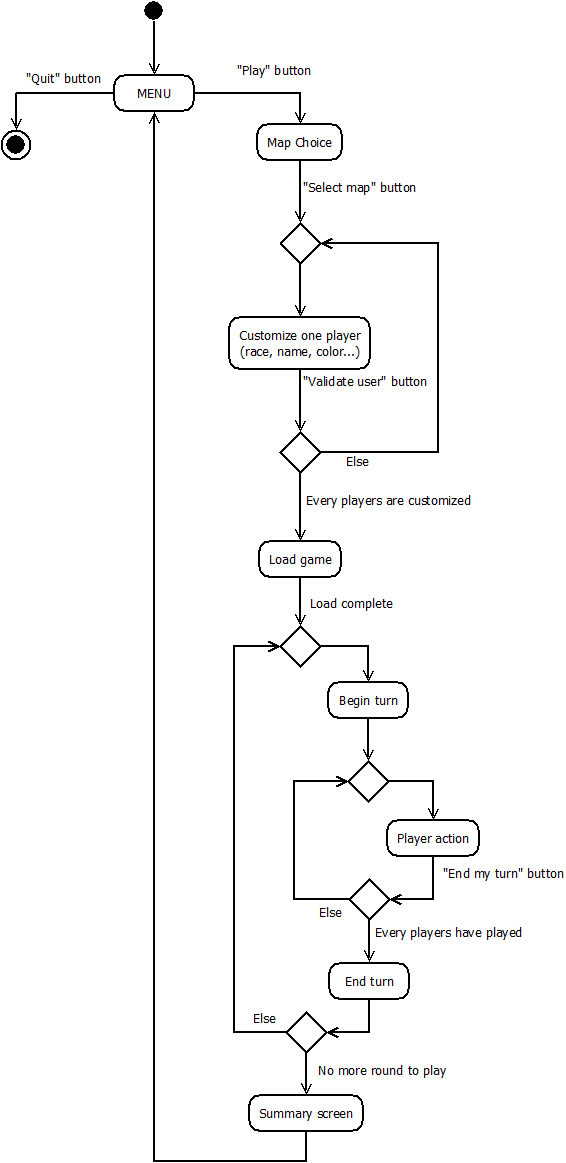
\includegraphics[width=5cm]{schemas/activity.png}
  \caption{Diagramme d'activité}
  \label{activity}
\end{figure}

\subsection{Créer ou charger une partie}

\paragraph{}
Lorsque les joueurs veulent lancer une partie, ils peuvent au choix en charger une existante ou en créer une nouvelle. Dans le cas d'une partie existante, la configuration des joueurs, la carte et les unités seront chargées afin de reprendre la partie là où elle en était. Par contre, si les joueurs décident de créer une nouvelle partie, alors ils devront pouvoir définir tous les paramètres nécessaires. Chacun leur tour, ils choisiront un nom, une race et s'accorderont sur une taille de carte. L'ensemble de ces usages sont présentés dans le diagramme de cas d'usage en Figure \ref{uc_game_creation}.

\begin{figure}[h]
  \centering
  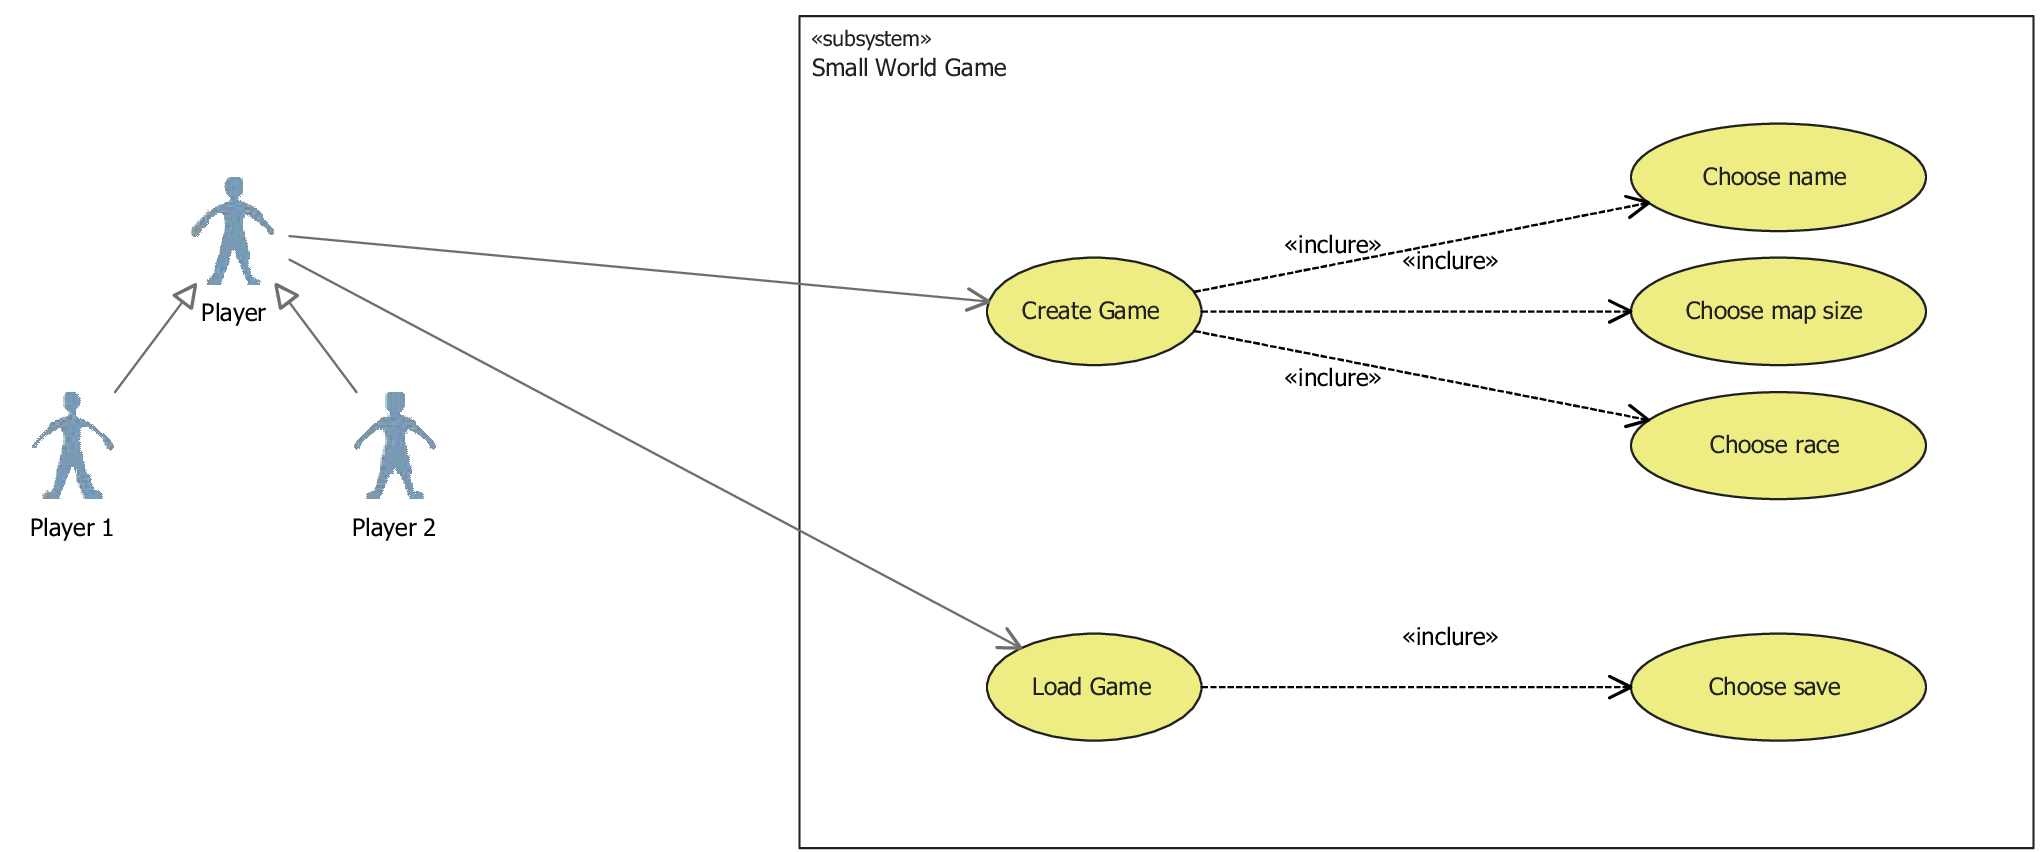
\includegraphics[width=8cm]{schemas/uc_game_creation.png}
  \caption{Diagramme de cas d'utilisation du lancement d'une partie}
  \label{uc_game_creation}
\end{figure}


\subsection{Déroulement d'un tour de jeu}

\paragraph{}
Lors d'un tour de jeu, le joueur pourra sélectionner ses unités, afin de leur demander de se déplacer ou d'attaquer. Chacune des unités aura 2 points d'action, et pourra donc potentiellement se déplacer et/ou attaquer dans la limite de ses points d'action disponibles. Les différentes actions possibles sont présentées dans la Figure \ref{uc_game_round}.

\begin{figure}[h]
  \centering
  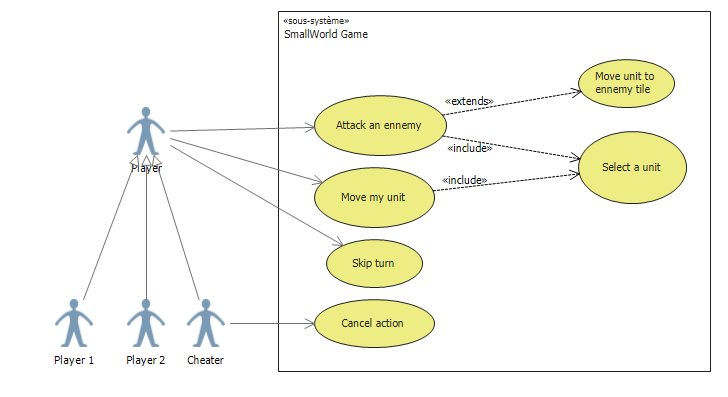
\includegraphics[width=8cm]{schemas/uc_game_round.png}
  \caption{Actions possibles lors d'un tour de jeu}
  \label{uc_game_round}
\end{figure}


\subsection{Cycle de vie d'une unité}

\paragraph{}
Les unités ont un cycle de vie particulier. Grâce aux états définis, nous pouvons imaginer associé un sprite différent en fonction de l'état de cette dernière. Par exemple, les unités dans l'état \og{} Full Life \fg{} utiliseront une image d'un personnage en bonne santé, celles dans l'état \og{} Hurt \fg{}  auront des blessures, et celles dans l'état \og{} Dead \fg{}  seront représentées par des tombes. Ces états permettent aussi de définir si l'unité peut se déplacer ou pas, etc.

\begin{figure}[!h]
  \centering
  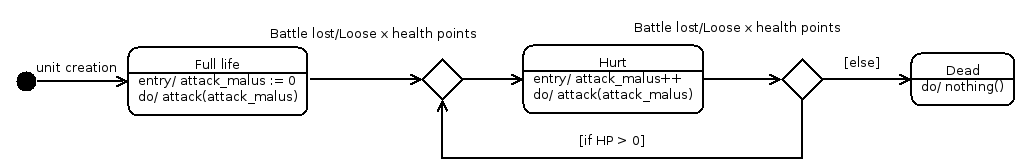
\includegraphics[width=13cm]{schemas/state-diagram.png}
  \caption{Cycle de vie d'une unité}
  \label{state-diagram}
\end{figure}


